% Created 2019-02-14 jue 16:00
% Intended LaTeX compiler: pdflatex
\documentclass[xcolor={usenames,svgnames,dvipsnames}]{beamer}
\usepackage[utf8]{inputenc}
\usepackage[T1]{fontenc}
\usepackage{graphicx}
\usepackage{grffile}
\usepackage{longtable}
\usepackage{wrapfig}
\usepackage{rotating}
\usepackage[normalem]{ulem}
\usepackage{amsmath}
\usepackage{textcomp}
\usepackage{amssymb}
\usepackage{capt-of}
\usepackage{hyperref}
\usepackage{color}
\usepackage{listings}
\usepackage{mathpazo}
\usepackage{gensymb}
\usepackage{amsmath}
\usepackage{chemarr}%flechas para reacciones químicas (SFER.tex)
\bibliographystyle{plain}
\AtBeginSubsection[]{\begin{frame}[plain]\tableofcontents[currentsubsection,sectionstyle=show/shaded,subsectionstyle=show/shaded/hide]\end{frame}}
\AtBeginSection[]{\begin{frame}[plain]\tableofcontents[currentsection,hideallsubsections]\end{frame}}
\usepackage[emulate=units]{siunitx}
\sisetup{fraction=nice, decimalsymbol=comma, retain-unity-mantissa = false}
\newunit{\wattpeak}{Wp}
\newunit{\watthour}{Wh}
\newunit{\amperehour}{Ah}
\usepackage{steinmetz}
\hypersetup{colorlinks=true, linkcolor=Blue, urlcolor=Blue}
\renewcommand{\thefootnote}{\fnsymbol{footnote}}
\beamertemplatenavigationsymbolsempty
\setbeamertemplate{footline}[frame number]
\setbeamercolor{alerted text}{fg=blue!50!black} \setbeamerfont{alerted text}{series=\bfseries}
\usetheme[hideothersubsections]{Goettingen}
\usecolortheme{rose}
\usefonttheme{serif}
\author{Oscar Perpiñán Lamigueiro}
\date{\url{http://oscarperpinan.github.io}}
\title{Solar Radiation on a Horizontal Plane}
\subtitle{Fundamentals of PV Engineering}
\hypersetup{
 pdfauthor={Oscar Perpiñán Lamigueiro},
 pdftitle={Solar Radiation on a Horizontal Plane},
 pdfkeywords={},
 pdfsubject={},
 pdfcreator={Emacs 26.1 (Org mode 9.2)}, 
 pdflang={Spanish}}
\begin{document}

\maketitle

\section{Motivation}
\label{sec:orgdcde097}
\begin{frame}[label={sec:org177e7ac}]{Solar Variability}
\begin{itemize}
\item \alert{Extraterrestrial} solar radiation is a \alert{deterministic process} (it depends on latitude, day of year, and time of day).
\item However, \alert{global radiation} is a \alert{stochastic (random) process} because of the interaction with the atmosphere:
\begin{itemize}
\item Time variability
\item Spatial variability
\end{itemize}
\end{itemize}

\begin{center}
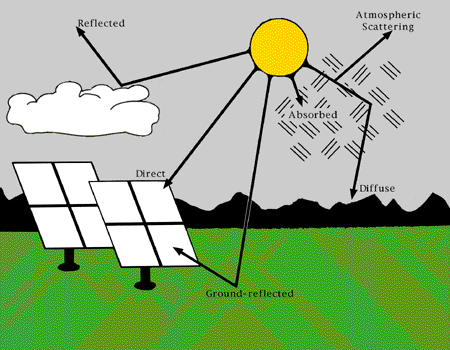
\includegraphics[height=0.4\textheight]{/home/oscar/github/esf/figs/SolarRadiationComponents_NREL.png}
\end{center}
\end{frame}

\begin{frame}[label={sec:orgcf26303}]{Long-term Estimations}
We are interested in \alert{long-term estimations} of the performance of PV systems in a definite location.

Solar radiation data sources must:
\begin{itemize}
\item \alert{capture the long-term behaviour} (interannual variability), and
\item be \alert{representative of the specified location} (spatial variability).
\end{itemize}
\end{frame}

\begin{frame}[label={sec:orgce5d1c6}]{Time Variability}
\begin{center}
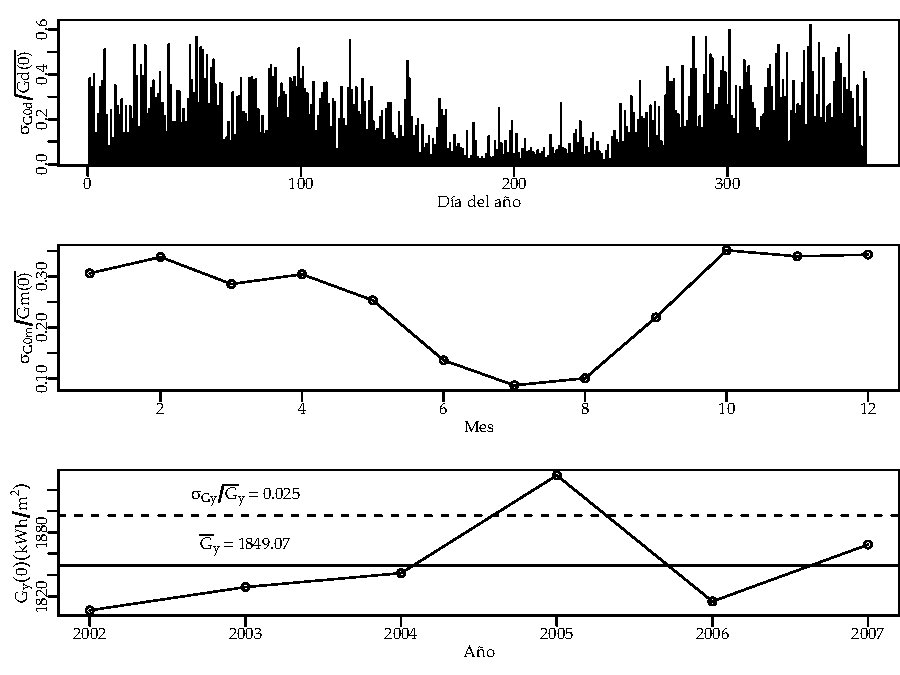
\includegraphics[height=0.4\textheight]{../figs/VariabilidadRadiacionDiario.pdf}
\end{center}

\begin{block}{Key concepts}
\begin{itemize}
\item Time variability \alert{increases with time resolution} (higher for daily values than for monthly averages).
\item Fluctuations are \alert{higher in winter than in summer}.
\item Reproducing \alert{long-term trends} requires \alert{long time series} (about 10 years length).
\end{itemize}
\end{block}
\end{frame}

\begin{frame}[label={sec:orgec2973c}]{Spatial Variability}
\begin{center}
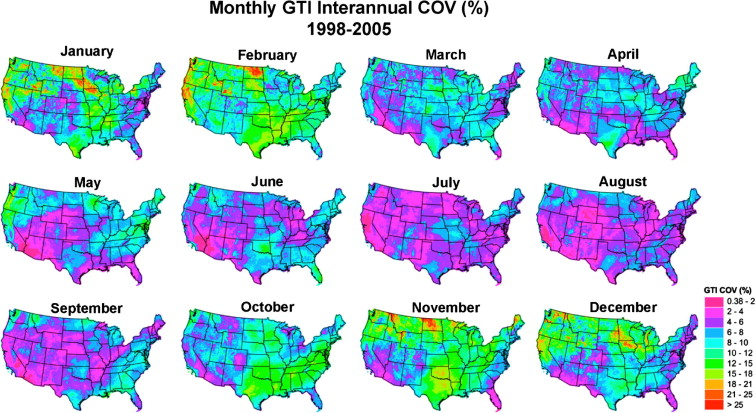
\includegraphics[height=0.4\textheight]{../figs/SpatialVariability.jpg}
\end{center}

\begin{block}{Key concepts}
\begin{itemize}
\item Spatial variability depends on the \alert{local climatology}.
\item Spatial variability is \alert{higher in winter than in summer} (for a same location).
\item Measurements are representative of nearby locations for a \alert{limited distance} (about 10 kms.)
\end{itemize}
\end{block}
\end{frame}

\begin{frame}[label={sec:org204fda5}]{Summary: Measurements requirements}
\begin{block}{}
\alert{Reliable} and \alert{representative} \alert{long-term estimations} of PV performance require:
\begin{itemize}
\item \alert{Nearby measurements}: \(\leq \SI{10}{km}\)
\item \alert{Long time series}: \(\simeq \SI{10}{years}\)
\end{itemize}
\end{block}
\end{frame}

\section{Data Sources}
\label{sec:org42d7db7}
\begin{frame}[label={sec:org1b7a437}]{Meteorological stations}
\begin{itemize}
\item Long time series.
\item High time resolution (\(\SI{1}{\min}\))
\item Low spatial resolution (point measurements).
\item Errors due to meter inaccuracy (no models required).
\end{itemize}

\begin{block}{Pyranometer}
\begin{center}
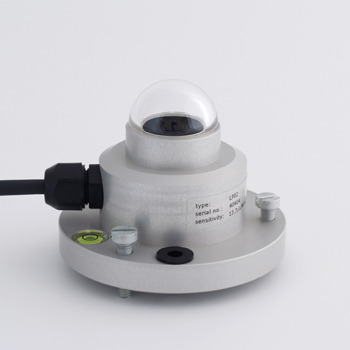
\includegraphics[height=0.5\textheight]{../figs/piranometro.jpg}
\end{center}
\end{block}
\end{frame}


\begin{frame}[label={sec:org5bfdece}]{Satellite imaging}
\begin{itemize}
\item Low time resolution (\(\SI{1}{hour}\) or \(\SI{1}{day}\)).

\item High spatial resolution (\(\SI{15}{km}\)).

\item Global solar radiation is estimated by processing images of the satellite radiometers.

\item Errors due model inaccuracy (radiation is estimated).
\end{itemize}
\begin{center}
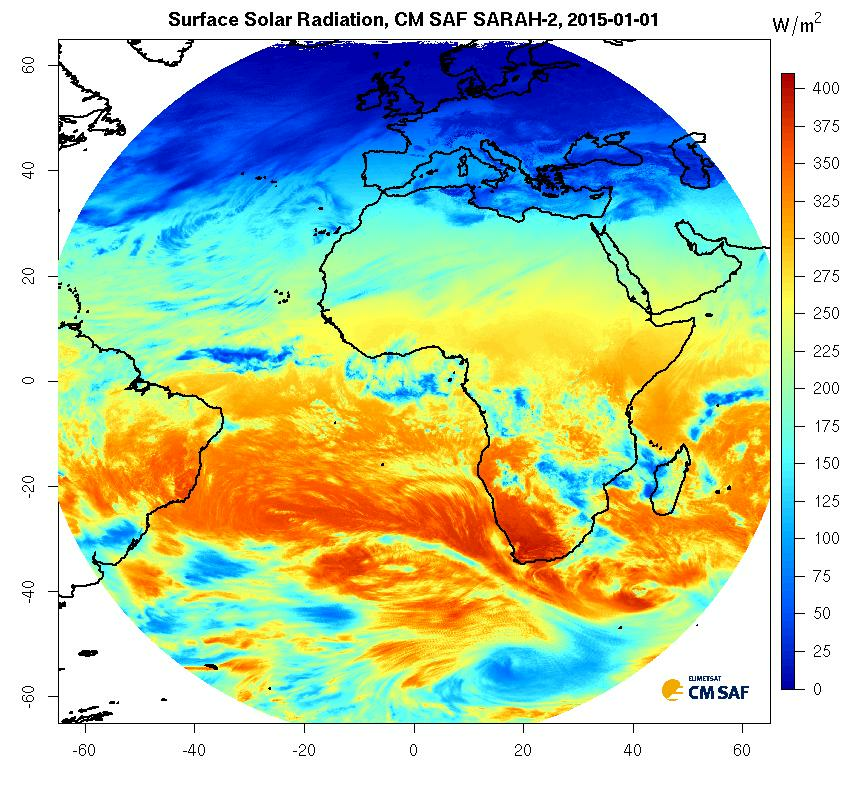
\includegraphics[height=0.5\textheight]{../figs/satellite.png}
\end{center}
\end{frame}

\begin{frame}[label={sec:orga2b1e0c}]{Hybrid methods}
Ground measurements merged with satellite estimations to increase spatial resolution:
\begin{itemize}
\item \alert{Inverse Distance Weighting (IDW)} (\(x_0\) is the point where the estimation is required, \(x_i\) are the points with measurements available, \(d\) is the distance between locations \(x_0\) and \(x_i\))
\[
\widehat{G}_d(x_0) = \frac{\sum_{i=1}^N w_i G_{d}(x_i)}{\sum_{i=1}^N w_i} 
\]

\[
  w_i = 1/d^2(x_0, x_i)
\]
\item \alert{Ordinary Kriging}
\item \alert{Kriging with External Drift (KED)}
\end{itemize}
\end{frame}

\begin{frame}[label={sec:org8eba65a}]{Data sources}
\url{https://github.com/oscarperpinan/mds/wiki}

\begin{itemize}
\item Meteorological Stations
\end{itemize}
\url{https://github.com/oscarperpinan/mds/wiki/stations}


\begin{itemize}
\item Satellite Estimations
\begin{itemize}
\item NASA: \url{https://github.com/oscarperpinan/mds/wiki/nasa}
\item CM SAF: \url{https://github.com/oscarperpinan/mds/wiki/cmsaf}
\end{itemize}

\item Hybrid estimations
\begin{itemize}
\item PVGIS: \url{https://github.com/oscarperpinan/mds/wiki/pvgis}
\item ADRASE: \url{https://github.com/oscarperpinan/mds/wiki/adrase}
\end{itemize}
\end{itemize}
\end{frame}

\section{Quality Control}
\label{sec:org8ee24e6}
\begin{frame}[label={sec:orgdb26589}]{Motivation}
Measurements must be \alert{filtered} and \alert{corrected} to remove erroneous data and outliers.
\begin{itemize}
\item Physical limits
\item Spatial coherence
\item Statistical analysis of deviations
\end{itemize}
\end{frame}


\begin{frame}[label={sec:orgfd844e9}]{Physical limits}
\begin{itemize}
\item \alert{Upper limit}: daily global irradiation cannot exceed extraterrestrial solar irradiation (daily clearness index\footnote{Clearness index is defined as the ratio \(K_{dT} = G_d(0) / B_{0d}(0)\).} cannot exceed 1).
\end{itemize}
\[
G_d(0) \leq B_{0d}(0)
\]

\[
  K_{dT} \leq 1
\]

\begin{itemize}
\item \alert{Lower limit}: clearness index must be higher than 0.03
\end{itemize}
\[
K_t = \frac{G_d(0)}{B_{0d}(0)} \geq 0.03
\]
\end{frame}

\begin{frame}[label={sec:orgebbed59}]{Spatial coherence}
Solar radiation measurements must be coherent between stations in a region.

\begin{itemize}
\item Measurements from a station should be compared with \alert{nearby stations} (for example, using IDW spatial interpolation)
\item Comparison must be established with \alert{aggregated values} (daily or monthly averages).
\end{itemize}
\end{frame}

\begin{frame}[label={sec:orge5a6736}]{Statistical Analysis of Deviations}
\begin{itemize}
\item Deviations, \(\mathbf{D}\), between Observations, \(\mathbf{O}\), and a Model, \(\mathbf{M}\) (or another set of observations):
\end{itemize}

\[
\mathbf{O} = \left\{ o_1 \dots o_n \right\}
\]

\[
\mathbf{M} = \left\{ m_1 \dots m_n  \right\}
\]

\[
\mathbf{D} = \mathbf{M} - \mathbf{O} =  \left\{ (m_1 - o_1) \dots (m_n - o_n)  \right\} = \left\{ d_1 \dots d_n  \right\}
\]
\end{frame}

\begin{frame}[label={sec:orgaeff53f}]{Accuracy and Precision}
\begin{center}
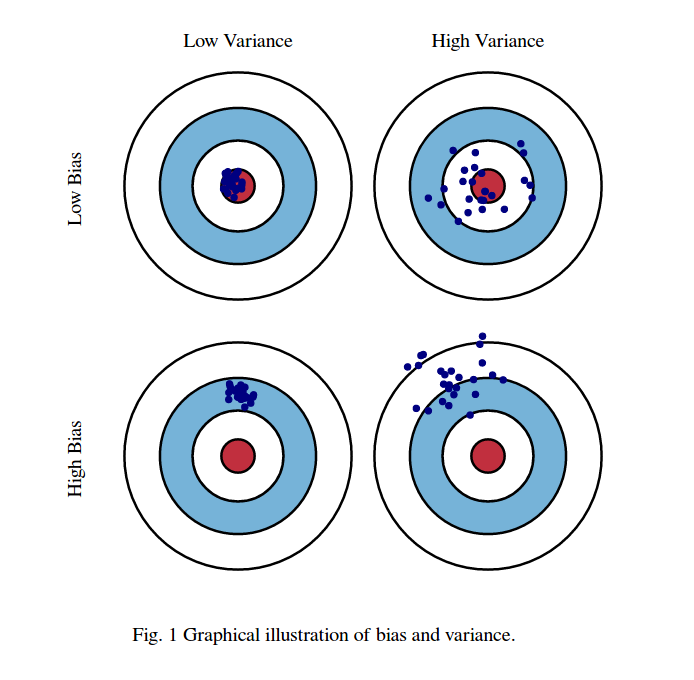
\includegraphics[height=0.8\textheight]{/home/oscar/github/esf/figs/bias-variance.png}
\end{center}

\url{http://scott.fortmann-roe.com/docs/BiasVariance.html}
\end{frame}

\begin{frame}[label={sec:org23ad10b}]{Metrics}
\begin{itemize}
\item Mean Bias Difference (MBD):
\end{itemize}
\[
MBE = \overline{\mathbf{D}} = \overline{\mathbf{M}} - \overline{\mathbf{O}} = \frac{1}{n} \sum_{i=1}^n (m_i - o_i)
\]

\begin{itemize}
\item Root Mean Square Difference (RMSD):
\end{itemize}
\[
RMSD = \left(\frac{1}{n} \sum_{i=1}^n d_i^2 \right)^{1/2} =  \left( \frac{1}{n} \sum_{i=1}^n (m_i - o_i)^2  \right)^{1/2}
\]

\begin{itemize}
\item Mean Absolute Deviation (MAD):
\end{itemize}

\[
MAD = \frac{1}{n} \sum_{i=1}^n \left|d_i\right| =  \frac{1}{n} \sum_{i=1}^n \left|m_i - o_i\right|
\]
\end{frame}
\end{document}